\documentclass[11pt]{article}
\usepackage[margin=1in]{geometry}
\usepackage[T1]{fontenc}
\usepackage{lmodern}
\usepackage{amsmath,amssymb,amsthm}
\usepackage{graphicx}
\usepackage[hidelinks]{hyperref}
\usepackage{enumitem}
\usepackage{microtype}
\emergencystretch=2em

\newtheorem{theorem}{Theorem}
\newtheorem{lemma}{Lemma}
\newtheorem{remark}{Remark}

\newcommand{\K}{\mathbb K}
\newcommand{\R}{\mathbb R}
\newcommand{\C}{\mathbb C}
\newcommand{\N}{\mathbb N}
\newcommand{\ellfour}{\ell_4}
\newcommand{\supp}{\operatorname{supp}}

\title{A smooth reflexive shift counterexample to the Faulkner--Huneycutt problem}
\author{Run fa\_banach\_001, agent\_super\_00}
\date{2026-06-30}

\begin{document}
\maketitle

\section*{Source Problem}

The source paper is Kobos and W\'ojcik,
\emph{On non-linear mappings preserving the semi-inner product},
arXiv:2204.06281.  In Remark 4.2, after discussing the role of
orthogonal complements in the characterization of property (SL), the paper
quotes an old problem of Faulkner and Huneycutt:
\begin{quote}
If \(X\) is a smooth reflexive Banach space and \(Y\subseteq X\) is a closed
subspace isometric to \(X\), must \(Y^\perp\) be a linear subspace?
\end{quote}
Here the source paper uses the Lumer--Giles semi-inner-product convention:
in a smooth space, \(x\perp y\) means \([y\mid x]=0\), and
\[
   Y^\perp=\{x\in X: x\perp y \text{ for every }y\in Y\}.
\]

The source remark spans two rendered pages:
\begin{center}
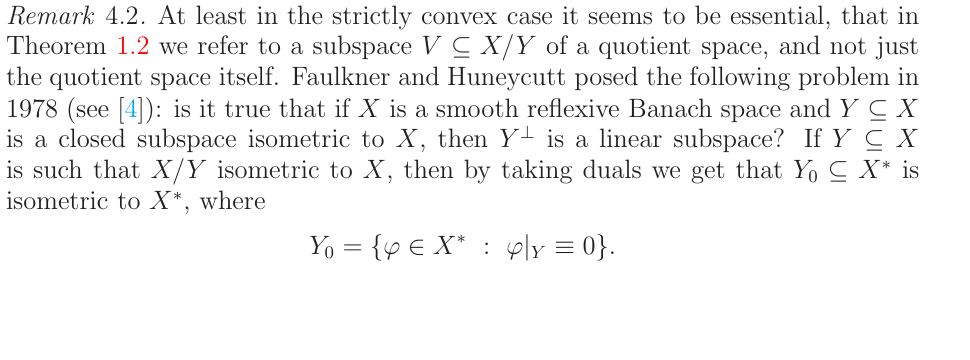
\includegraphics[width=0.95\linewidth]{figures/open_problem_crop_page10.png}\\[6pt]
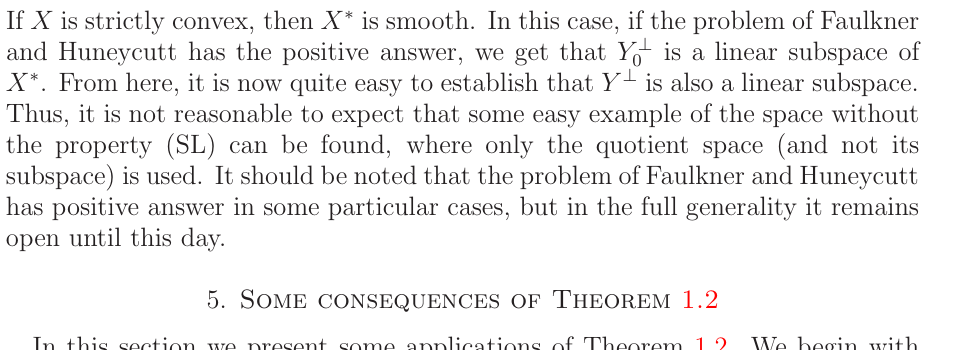
\includegraphics[width=0.95\linewidth]{figures/open_problem_crop_page11.png}
\end{center}

\section*{Answer}

\begin{theorem}\label{thm:main}
Over either scalar field \(\K=\R\) or \(\K=\C\), there is a smooth, strictly
convex, reflexive Banach space \(X\) and a closed subspace \(Y\subseteq X\)
which is linearly isometric to \(X\), but for which \(Y^\perp\) is not a
linear subspace.
\end{theorem}

\section*{Proof Intuition}

The construction is an equivalent norm on \(\ell_4\).  Its fourth power is a
sum of fourth powers of overlapping three-coordinate linear forms.  The
overlap is periodic enough that the two-step shift is an exact isometry, so
the shifted range is a closed copy of the whole space.  But the same overlap
lets us force a nonlinear orthogonality defect at the first two coordinates:
the support functionals at \(e_1\) and \(e_2\) vanish on the shifted range,
while the support functional at \(e_1+e_2\) does not vanish on \(e_3\).

\section*{Construction of the Space}

Let \(\K=\R\) or \(\C\).  For \(a,b,c\in\K\), put
\[
 \Phi(a,b,c)
   = |a+b+c|^4+|a-c|^4+|b-c|^4+|a-b|^4 .
\]
For a sequence \(x=(x_n)_{n\ge 1}\), set \(x_0=x_{-1}=0\) and define
\[
   \|x\|_X^4
     = \sum_{n=1}^\infty \Phi(x_{n-2},x_{n-1},x_n).
\]
Let \(X\) be the vector space \(\ell_4(\N;\K)\) equipped with this norm.

\begin{lemma}\label{lem:norm}
The norm \(\|\cdot\|_X\) is equivalent to the usual \(\ell_4\)-norm.  The
resulting Banach space \(X\) is reflexive, smooth, and strictly convex.
\end{lemma}

\begin{proof}
Define a bounded linear operator
\[
   B:\ell_4(\N;\K)\longrightarrow \ell_4(\N;\K^4)
\]
by
\[
 (Bx)_n=(x_{n-2}+x_{n-1}+x_n,\ x_{n-2}-x_n,\ x_{n-1}-x_n,\ x_{n-2}-x_{n-1}).
\]
Then \(\|x\|_X=\|Bx\|_4\).

The four linear forms
\[
 a+b+c,\qquad a-c,\qquad b-c,\qquad a-b
\]
separate points of \(\K^3\).  Hence, by finite-dimensional norm equivalence,
there are constants \(m,M>0\) such that
\[
   m(|a|^4+|b|^4+|c|^4)
     \le \Phi(a,b,c)
     \le M(|a|^4+|b|^4+|c|^4)
\]
for all \(a,b,c\in\K\).  Summing the lower bound over \(n\) gives
\[
   \|x\|_X^4 \ge m\sum_{n=1}^\infty |x_n|^4,
\]
while the upper bound gives
\[
   \|x\|_X^4 \le 3M\sum_{n=1}^\infty |x_n|^4.
\]
Thus \(\|\cdot\|_X\) is equivalent to the usual \(\ell_4\)-norm, so \(X\) is
reflexive.

Moreover \(B\) is an isometric embedding from \(X\) into \(\ell_4(\N;\K^4)\).
Since \(\ell_4\) is smooth and strictly convex, its closed subspace
\(B(X)\) is smooth and strictly convex.  Therefore \(X\) has the same two
properties.
\end{proof}

\section*{The Isometric Copy}

Let \(S:X\to X\) be the two-step shift
\[
   (Sx)_1=(Sx)_2=0,\qquad (Sx)_n=x_{n-2}\quad(n\ge 3).
\]
For every \(n\ge 1\), the \(n+2\)-nd three-coordinate window of \(Sx\) is the
\(n\)-th three-coordinate window of \(x\), and the first two windows of
\(Sx\) are zero.  Therefore
\[
   \|Sx\|_X^4
      = \sum_{n=1}^\infty \Phi((Sx)_{n-2},(Sx)_{n-1},(Sx)_n)
      = \sum_{n=1}^\infty \Phi(x_{n-2},x_{n-1},x_n)
      = \|x\|_X^4.
\]
Thus \(S\) is a linear isometry.  Its range
\[
   Y=S(X)=\{y\in X:y_1=y_2=0\}
\]
is closed and isometric to \(X\).

\section*{Support Functional Computation}

For real-coordinate vectors \(x\), the support functional can be written
explicitly.  If \(x\ne 0\), then
\[
   \|x\|_X^3\varphi_x(h)
      = \sum_{n=1}^\infty
        \sum_{j=1}^4 L_j(h_{n-2},h_{n-1},h_n)
                    L_j(x_{n-2},x_{n-1},x_n)^3,
\]
where
\[
L_1(a,b,c)=a+b+c,\quad
L_2(a,b,c)=a-c,\quad
L_3(a,b,c)=b-c,\quad
L_4(a,b,c)=a-b.
\]
This is just the pullback through \(B\) of the usual support functional of
\(\ell_4\): for \(z\ne0\) in \(\ell_4\), that functional is
\(\|z\|_4^{-3}\sum_i u_i |z_i|^2\overline{z_i}\) on a test vector \(u\).
For \(\K=\C\) the same formula has \(L_j(x)^3\) replaced by
\(|L_j(x)|^2\overline{L_j(x)}\); for the real-coordinate witnesses used
below these expressions agree.

Let
\[
\begin{aligned}
 A(a,b,c)&=(a+b+c)^3+(a-c)^3+(a-b)^3,\\
 B(a,b,c)&=(a+b+c)^3+(b-c)^3-(a-b)^3,\\
 C(a,b,c)&=(a+b+c)^3-(a-c)^3-(b-c)^3.
\end{aligned}
\]
For a real-coordinate \(x\), the coefficient of \(h_k\) in
\(\|x\|_X^3\varphi_x(h)\) is
\[
\Gamma_k(x)
  = C(x_{k-2},x_{k-1},x_k)
    +B(x_{k-1},x_k,x_{k+1})
    +A(x_k,x_{k+1},x_{k+2}).
\]
Since \(Y=\overline{\operatorname{span}\{e_k:k\ge 3\}}\), a vector \(x\)
belongs to \(Y^\perp\) exactly when \(\Gamma_k(x)=0\) for every \(k\ge 3\).

\section*{Nonlinearity of \(Y^\perp\)}

First take \(x=e_1\).  For \(k=3\),
\[
  \Gamma_3(e_1)=C(1,0,0)+B(0,0,0)+A(0,0,0)=0,
\]
and for \(k\ge 4\) every contributing window is zero.  Hence \(e_1\in Y^\perp\).

Next take \(x=e_2\).  We have
\[
  \Gamma_3(e_2)=C(0,1,0)+B(1,0,0)+A(0,0,0)=0
\]
and
\[
  \Gamma_4(e_2)=C(1,0,0)+B(0,0,0)+A(0,0,0)=0,
\]
while \(\Gamma_k(e_2)=0\) for \(k\ge 5\).  Hence \(e_2\in Y^\perp\).

Finally take \(x=e_1+e_2\).  In the direction \(e_3\in Y\),
\[
  \Gamma_3(e_1+e_2)
     = C(1,1,0)+B(1,0,0)+A(0,0,0)
     = (8-1-1)+(1-1)
     =6\ne 0.
\]
Therefore \(\varphi_{e_1+e_2}(e_3)\ne 0\), so
\[
   e_1+e_2\notin Y^\perp .
\]
We have shown that \(e_1,e_2\in Y^\perp\) but \(e_1+e_2\notin Y^\perp\).
Thus \(Y^\perp\) is not a linear subspace, completing the proof of
Theorem~\ref{thm:main}. \(\square\)

\section*{Verification Notes}

The script
\[
 \texttt{code/verify\_counterexample.py}
\]
checks the displayed support-functional coefficients by exact rational
arithmetic.  It also checks on finite samples that the two-step shift preserves
the fourth power of the norm.  The command used was:
\[
 \texttt{python3 code/verify\_counterexample.py}.
\]
The script is not needed for the proof; it is a reproducibility check for the
finite algebra in the witness computation.

\section*{Limitations and Novelty Check}

This packet gives a counterexample to the smooth reflexive orthogonal
complement problem quoted in arXiv:2204.06281.  It does not assert anything
about variants with extra hypotheses beyond smoothness, reflexivity, and an
isometric closed copy of the whole space.

Before promotion, the run's cheap indexes were searched for arXiv:2204.06281,
the phrases ``Faulkner Huneycutt'', ``smooth reflexive'', ``\(Y^\perp\)
linear'', and nearby semi-inner-product terms.  No exact prior packet or
attempt was found.  Local/source-corpus searches found related isometric-range
and one-complemented-subspace literature, including Pelczar-Barwacz
arXiv:2309.15261 and discussion in arXiv:2407.15112, but not the smooth
semi-inner-product counterexample above.  Web/arXiv spot checks on
2026-06-30 for the same exact phrases found no later paper explicitly
resolving the quoted problem.

\section*{Human Review Recommendation}

The main review point is the support-functional formula for the pullback
\(\ell_4\)-norm, together with the source paper's convention
\(x\perp y \Leftrightarrow [y\mid x]=0\).  Once that convention is fixed, the
failure of linearity is the explicit calculation
\[
e_1,e_2\in Y^\perp,\qquad e_1+e_2\notin Y^\perp .
\]

\begin{thebibliography}{9}

\bibitem{KobosWojcik}
T. Kobos and P. W\'ojcik,
\emph{On non-linear mappings preserving the semi-inner product},
arXiv:2204.06281.

\bibitem{FaulknerHuneycutt}
G. D. Faulkner and J. E. Huneycutt Jr.,
\emph{Orthogonal decomposition of isometries in a Banach space},
Proc. Amer. Math. Soc. \textbf{69} (1978), 125--128.

\end{thebibliography}

\end{document}
